%-----------------------------------------------------------------------------%
%                                                                             %
%                                lecture1.tex                                 %
%                                                                             %
%                               Achim Ibenthal                                %
%                                                                             %
%                                                                             %
% CONTENT:             Vorlesung Lecture 1                                    %
%                                                                             %
% REVISION HISTORY     04-AUG-06: Initial Version                             %
%                      26-AUG-06: Update new Beamer layout + MiKTeX 2.7       %
%                                                                             %
%-----------------------------------------------------------------------------%

%-----------------------------------------------------------------------------%
%                             Lesson Title + ToC                              %
%-----------------------------------------------------------------------------%


\mode<presentation>{

   % Change Title Page Content HERE
   \title{Lecture 1}
   \TitleTextBox[Ziel:]{Verst�ndnis Lecture 1}

   % Insert a title slide
   \frame{\clockinit\titlepage}
}


%-----------------------------------------------------------------------------%
%                              Nutzungsrichtlinie                             %
%-----------------------------------------------------------------------------%

\slideonly{
   \begin{frame}[c]
   \frametitle{Nutzungsrichtlinie}

   \begin{beamercolorbox}[rounded=true,shadow=true,sep={0.5ex}]
         {block body alerted}\slup{1}
   
   \parbox[t]{0.980\hsize}{\footnotesize\docnutzung\normalsize}
   
   \slup{0}
   \end{beamercolorbox}

   \end{frame}
}

\scrnp % Script: new page for each new section


%-----------------------------------------------------------------------------%
%                                 Section 1                                   %
%-----------------------------------------------------------------------------%

\section{Section 1}
\label{sec:sec1}


%-----------------------------------------------------------------------------%
%                          Subsection 1 of Section 1                          %
%-----------------------------------------------------------------------------%

\subsection[Section 1 ]{Zero-shot learning}
\label{ssec:sec1a}


%-----------------------------------------------------------------------------%

\begin{frame}%[allowframebreaks,fragile]
\frametitle{zero-shot learning}

	\ndef{def:<label>}{Zero-shot learning}{
	aims to train a model that can classify objects of unseen classe(target domain) via transfering knowledge obteined from other seen classes(source domain) with the help of semantic information
	\filledend}
\nblock 
{Problem}
{more challenging scenario with no data for unseen classe,relying solely on descriptions and transfered knowledge from seen classes.}

\ndef{def:<label>}{Generalized Zero-shot learning}{
	more realistic scenario with some data for seen classes to help classify unseen classes using description and visual representation
	\filledend}

\end{frame}

\begin{frame}%[allowframebreaks,fragile]
	\frametitle{Generalized Zero-Shot Learning (GZSL)}
		\begin{center}
		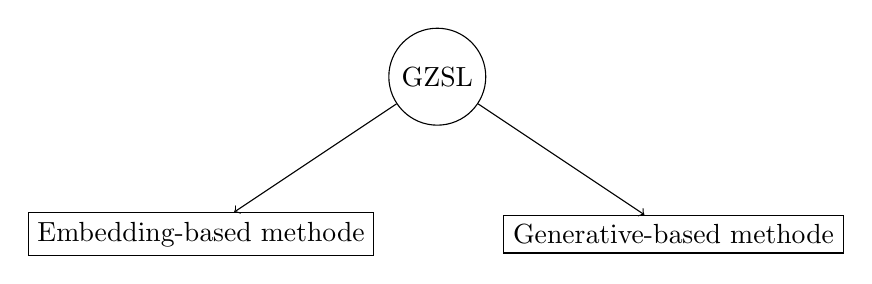
\begin{tikzpicture}
			\node[draw, circle] (model) at (0,0) {GZSL};
			\node[draw, rectangle] (methode1) at (-3,-2) {Embedding-based methode};
			\node[draw, rectangle] (methode2) at (3,-2) {Generative-based methode};
			\draw[->] (model) -- (methode1);
			\draw[->] (model) -- (methode2);
		
		\end{tikzpicture}
		\ndef{def:<label>}{Embedding-based methode}{
		learn an embedding space whether visual-semantic ,semantic-visual, commun/latent or a combination of them (Graph-Based, Autoencoder-Based, Meta-Learning-Based, Compositional Learning and Bidirectional Learning-Based)
			\filledend}
			

	\end{center}
	
	
\end{frame}

\begin{frame}%[allowframebreaks,fragile]
	\frametitle{Generalized Zero-Shot Learning (GZSL)}
	\begin{center}
		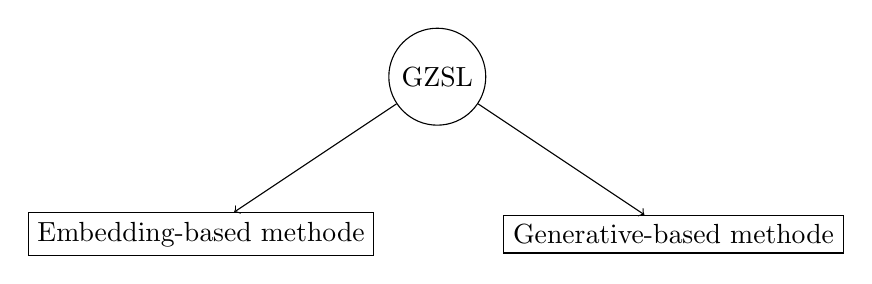
\begin{tikzpicture}
			\node[draw, circle] (model) at (0,0) {GZSL};
			\node[draw, rectangle] (methode1) at (-3,-2) {Embedding-based methode};
			\node[draw, rectangle] (methode2) at (3,-2) {Generative-based methode};
			\draw[->] (model) -- (methode1);
			\draw[->] (model) -- (methode2);
			
		\end{tikzpicture}
		\ndef{def:<label>}{Generative-based methode}{
		convert GZSL into a conventional supervised learning problem by generating visual features for the unseen classes (Generative Adverserial Network and Variational AutoEncoder (VAE))
			\filledend}
		
		
	\end{center}
	
	
\end{frame}


\begin{frame}%[allowframebreaks,fragile]
\frametitle{Generalized Zero-Shot Learning (GZSL)}

		
	\begin{table}[h]
			\centering
			\begin{tabular}{|m{2cm}|m{4cm}|m{4cm}|}
				\hline
				& \textbf{Embedding-based } & \textbf{Generative-based} \\
				\hline
				\textbf{Adventage} & 
				\begin{itemize}
					\item can be effective for simple objects
					
				\end{itemize}
				& 
				\begin{itemize}
					\item can potentially handle complex object better by creating realistic visual representation
				
				\end{itemize} \\
				\hline
				\textbf{Desadvantage} & 
				\begin{itemize}
					\item suffer from the seen classes overfitting problem due to the data imbalance nature of ZSL
				
				\end{itemize}
				& 
				\begin{itemize}
		           \item the quality of generated images can be a chalange and impact classification accuracy
				\end{itemize} \\
				\hline
			\end{tabular}
			\caption{Advantage and Desadvantage of GZSL methodes}
			\label{table:adv_disadv}
		\end{table}
\end{frame}




\begin{frame}%[allowframebreaks,fragile]
	\frametitle{Generalized Zero-Shot Learning (GZSL)}
	\begin{center}
		\begin{tikzpicture}
			\node[draw, rectangle split draw splits ] (model) at (0,-2) {Hybrid methode};
			\node[draw, rectangle] (methode1) at (-3,0) {Embedding-based methode};
			\node[draw, rectangle] (methode2) at (3,0) {Generative-based methode};
			\draw[->] (model) -- (methode1);
			\draw[->] (model) -- (methode2);
			
		\end{tikzpicture}
		
			\begin{itemize}
			\item The Constractive Embedding for generalized zero-Shot learning paper proposes a hybrid GZSL framwork that comnbines the two models 
		\end{itemize}
	
		\ndef{def:<label>}{Constractive Embedding}{
			is integrated into hybrid GZSL with the goal to construct embeddings that facilitate the recognition of unseen classes by leveraging the relationships and similarities between seen and unseen classes
			\filledend}
			
			
		
		
	\end{center}
	
	
\end{frame}

\begin{frame}%[allowframebreaks,fragile]
	\frametitle{Generalized Zero-Shot Learning (GZSL)}
	\begin{center}
				\ndef{def:<label>}{Constractive Embedding}{
			is integrated into hybrid GZSL with the goal to construct embeddings that facilitate the recognition of unseen classes by leveraging the relationships and similarities between seen and unseen classes
			\filledend}
		
		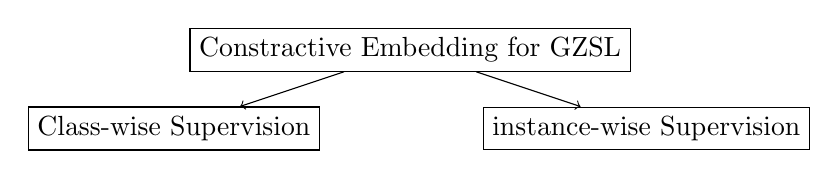
\begin{tikzpicture}
			\node[draw, rectangle] (model) at (0,0) {Constractive Embedding for GZSL};
			\node[draw, rectangle] (methode1) at (-3,-1) {Class-wise Supervision };
			\node[draw, rectangle] (methode2) at (3,-1) {instance-wise Supervision };
			
			\draw[->] (model) -- (methode1);
			\draw[->] (model) -- (methode2);
			
		\end{tikzpicture}
			\ndef{def:<label>}{Class-wise and instance-wise supervision }{
			Class-wise Supervision is to classify the membership and the instance-wise Supervision is to identify the similarities or the differenz between individual image .
			\filledend}
		
	
		
		
		
	\end{center}
	
	
\end{frame}

%-----------------------------------------------------------------------------%
%                                  Section 2                                  %
%-----------------------------------------------------------------------------%

\section{Section 2}
\label{sec:sec2}


%-----------------------------------------------------------------------------%
%                          Subsection 1 of Section 1                          %
%-----------------------------------------------------------------------------%

\subsection[Subsection 1]{One-Shot learning }
\label{ssec:sec2a}



%-----------------------------------------------------------------------------%
%                          Section2                          %
%-----------------------------------------------------------------------------%


\begin{frame}%[allowframebreaks,fragile]
	\frametitle{One-shot learning}
	
	
		\ndef{def:<label>}{One-shot learning }{
		aims to identifying within a target image all object instance of the same class,implied by a query image patch with the problem that its label and its respective exemple are not available in the training data .
			\filledend}
			\begin{center}
				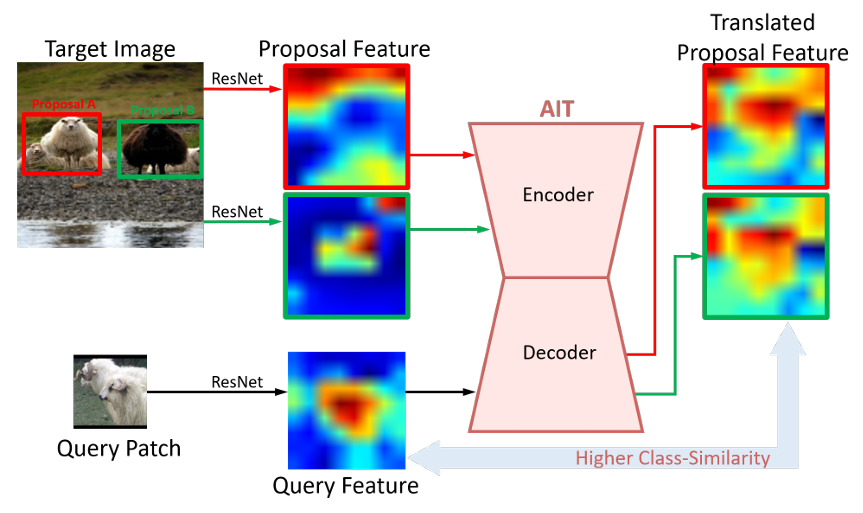
\includegraphics[width=0.5\textwidth]{script/AIT.PNG}
			\end{center}
			\ndef{def:<label>}{Adaptive Image Transformer }{
				AIT module aims to compare the features of regions or abjects in the Target Image based on the language translation process:
				\filledend}
		
		
	
	
	
\end{frame}

\begin{frame}%[allowframebreaks,fragile]
	\frametitle{One-shot learning}
		
	\begin{itemize}
		\item AIT can adaptively represent each region proposal so that the similarity with the query can be evaluated ,that module uses an attention based encoder-decoder architecture to simultaneausly explore intra-coder and inter-coder
		\item encoder converts the inpute data (e.g. features of objects proposals) into internal representation. 
		\item decoder generates the output from this internal representation(e.g. class similarity between proposals and the query image.)
		\item Intra-coder attention refers to the relationships within a single coder, for exemple the relationship and the importance between different parts of a single image proposal to generate a better internal representation.
		\item Inter-coder attention examines the relationshipes between different coders. the model learns how each proposal is related the query image,which help to better judge class similarity
		

	\end{itemize}
	

	
	
\end{frame}


\begin{frame}%[allowframebreaks,fragile]
	\frametitle{One-shot learning}
	\begin{itemize}
		\item sparse attention mecanism help the model focus on the most important part of the data.
		
		\vspace{10ex}
		
\item[Evaluation] Higher mAP (Mean Average Precision) means more accurately detecting and classifying abjects from all classes .
	\end{itemize}
\end{frame}


\begin{frame}%[allowframebreaks,fragile]
	\frametitle{One-shot learning in Text-to-video generation}
	\begin{center}
		\begin{tikzpicture}[auto, node distance=2cm,>=latex']
			% Nodes
			\node[draw, rectangle split draw splits] (model) at (0,0) {Generation of videos from text};
			\node[draw, rectangle] (methode1) at (-3,-2) {Traditional approaches};
			\node[draw, rectangle] (methode2) at (3,-2) {One-Shot Video Tuning};
			
			% Explanations
			\node[align=left, below] at (methode1.south) {extensive and large \\ Text-video datasets are \\ requires to train a model};
			\node[align=left, below] at (methode2.south) {learns to generate videos \\ based on just one exemple \\ instruction and its corresponding \\ video };
			
			% Connections
			\draw[->] (model) -- (methode1);
			\draw[->] (model) -- (methode2);
		\end{tikzpicture}
			\end{center}
	
\end{frame}

\begin{frame}[fragile]
	\frametitle{One-shot learning in Text-to-video generation}
	
	\begin{exampleblock}{One-shot video tuning}
		\begin{verbatim}
		" a man is running on the beach" and a single video that 
		shows exactly this scene .
		\end{verbatim}
			
		\vspace{-5ex}
		\begin{enumerate}
			\item pretraining phase : learns to generate images from text description 
			\item learn how to translate the specific text description into motion pictures, das model learns that the beach describe a specific environment and a man has a certain shape
			\item generating similar video : generation of videos based on different text description with different scenario , event though had learnt just from one exemple
		\end{enumerate}
	\end{exampleblock}
	
		\begin{exampleblock}{Application}
	
		\begin{enumerate}
			\item object editing . 
			\item Background changing .
			\item generating similar video : generation of videos based on different text description with style transfer for exemple from real-worls into comic style.
		\end{enumerate}
	\end{exampleblock}
	

	
\end{frame}

%-----------------------------------------------------------------------------%
%                                  Section 2                                  %
%-----------------------------------------------------------------------------%

\section{Section 3}
\label{sec:sec3}


%-----------------------------------------------------------------------------%
%                          Subsection 1 of Section 1                          %
%-----------------------------------------------------------------------------%

\subsection[Subsection 1]{Few-Shot learning }
\label{ssec:sec3a}


\begin{frame}%[allowframebreaks,fragile]
	\frametitle{Few-shot learning}
	
	
	\ndef{def:<label>}{Few-shot learning }{
		aims to learn information about Data from very limited number of training data when the collecting a large dataset is impossible .
		\filledend
		}
			\nblock	{Problem}
		{more challenging for few-shot learning in traditional neural network is the low effectiveness with very limited labled data (e.g. overfitting ).}
		
		\ndef{def:<label>}{Overfitting }{
			A model overfits the training data when it describes features that arise from noise or variance in the data, rather than the underlying distribution from which the data were drawn. Overfitting usually leads to loss of accuracy on out-of-sample data.
			
			\filledend}

	
	
	
	
	
\end{frame}



\begin{frame}%[allowframebreaks,fragile]
	\frametitle{Few-shot learning}
	
	
	\ndef{def:<label>}{A few-shot learning model based on Siamese Convolutional Neural Network (CNN) }{
	A Siamese CNN consists of two identical subnetworks that work in parallel and share the same weights. This network compares two inputs and learns whether they belong to the same class or not. By comparing sample pairs, the model can learn more robust and generalizable features, which reduces overfitting.
		\filledend}
	 
	
\end{frame}


\begin{frame}%[allowframebreaks,fragile]
	\frametitle{Few-shot learning}
	
	
	\begin{center}
	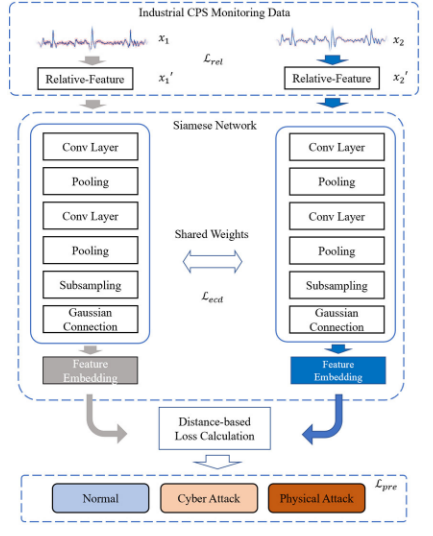
\includegraphics[width=0.4\textwidth]{script/seamse.PNG}
\end{center}
\begin{itemize}
	\item pooling layer helps in reducing high dimensional convolutional features .
	\item Conv layal to identify from the imput data the importent features using edges and textures detection .
	\item two combinations of convolution layer and
	pooling layer are introduced to extract feature embeddings
\end{itemize}

	
	
	
	
	
\end{frame}



\begin{frame}%[allowframebreaks,fragile]
	\frametitle{Few-shot learning}
	
	
\begin{itemize}
	\item the distance between these two feature embeddings will be calculated to identify whether these two
	input samples belong to the same class.
 

\end{itemize}
	
	
\end{frame}

\begin{frame}%[allowframebreaks,fragile]
	\frametitle{Few-shot learning}
	
	
	\ndef{def:<label>}{Few-Shot Hyperspectral Image Classification  }{
	Hyperspectral Image Classification : The objects are classified by its HyperSpectrum .
		\filledend}
			\nblock	{Problem}
		{Current hyperspectral image classification assumes that a predefined classification system is closed and complete, and there are no unknown or novel classes in the unseen data. When a new class appears, it will be  interpreted as an error ,what is not the case .}
		
		\ndef{def:<label>}{MDL4OW(multitask deep learning)}{
			method that simultaneously conducts classification and reconstruction in the open world .The reconstructed data are compared with the original data; those failing to be reconstructed are considered unknown classes .
			
			\filledend}
			
	
\end{frame}

\begin{frame}%[allowframebreaks,fragile]
	\frametitle{Few-shot learning}
	
	
	\begin{center}
		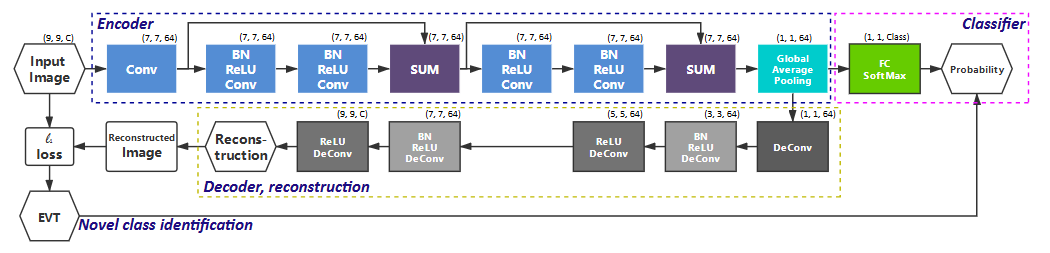
\includegraphics[width=1.1\textwidth]{script/hyperspectrale.PNG}
	\end{center}
	\begin{itemize}
		\item the encoder/features extractor get from the inpute image the proposal features using Pooling and convolution layal .
		\item after extracting the latent features the function softmax serves as the classifier and outputes the probability to the known classes .
		\item the reconstruction task uses the deconvolutional layers to increase the spatial dimonsion of the latent features gradually, the output should be similar to the input data .
	\end{itemize}
	

\end{frame}


%-----------------------------------------------------------------------------%
%                              Exercises Section 1                            %
%-----------------------------------------------------------------------------%

\subsection[�bungen]{�bungen \scriptonly{zu Abschnitt \ref{sec:sec1}}}
\label{ssec:exercisesec1}


%-----------------------------------------------------------------------------%









\begin{frame}[c,allowframebreaks]
	\slideonly{\frametitle{Application : Generative-based methode(WGAN) }}
	
	
			\begin{itemize}
			\item The application is coming to solve the problem that we dont have enough data from the unseen classes so the generative-based mothod is coming to generate more data . 
			\item [Objective] The ability of the model to generate new feature vectors that represent unseen classes allows to extend classification to unseen classes.	
		    \end{itemize}
		
	\end{frame}
	
	

	\begin{frame}[c,allowframebreaks]
		\slideonly{\frametitle{Application : Generative-based methode(WGAN) }}
		
	
	
	
		\ndef{def:<label>}{Generative space}{
		By training a generative adverserial network(GAN), they learn to generate new features vectors.
		\filledend}
         \begin{itemize}	
                  \item	Our application is about a simplified [AWA2] databases instead of using raw images, extracting features that present the image in a compact yet informative form.
                  \item[AWA2] contains 30475 images cotegorized into 40 seen classe for training and 10 additional unseen  classes for test.
                  \item[Attribute] AH-splits.mat contains the attribute data,every class is represented by a vector with 85 attributes 
                 \item The values can be benary or float, which can represent the strength of these properties
                  \item[Features] res101.mat representes  the processed image characteristics for each image in AWA2 database, res101 has the ability to present images in a very compact and information-rich manner, rather than raw images that are data-wise heavy.the features are stored as vectors: each vector represents an image and contains a numerical description of the image e.g. shapes, colors, textures and structures .
                 
       \end{itemize}
       
	
\end{frame}
	
	
	\begin{frame}[c,allowframebreaks]
		\slideonly{\frametitle{Application : Generative-based methode(WGAN) }}
		
		
	
		 \nblock	{Problem}
		{Let $S = \{(x_i^s, a_i^s, y_i^s)_{i=1}^{N_s} | x_i^s \in X^s, a_i^s \in A^s, y_i^s \in Y^s \}$ and
			$U = \{(x_j^u, a_j^u, y_j^u)_{j=1}^{N_u} | x_j^u \in X^s, a_j^u \in A^s, y_j^u \in Y^s \}$ represent  the seen and unseen class data sets, respectively, where $x_i^s, x_j^u \in \mathbb{R}^D$ indicate the $D$-dimensional images (visual features) in the feature space $X^s$ that can be obtained using a pre-trained deep learning model such as ResNet.
			$a_i^s$,$a_j^u \in \mathbb{R}^K $   indicate the
			K-dimensional semantic representations (attributes vector) in the semantic space $A$. $Y_s = \{y_1^s, ...,y_{40}^s\}$ and $Y_u = \{y_1^u, ...,y_{10}^u\}$ indicate the label sets of both seen and unseen classes in the label space $Y$ where 40 and 10  are
			the number of  seen and unseen classes, $\mathcal{Y}=Y^s \cap Y^s$  denotes
			the union of both seen and unseen classes and	 $\emptyset=Y^s \cup Y^s$ 		
			
			}
			
			
		
	\end{frame}
	
	
		\begin{frame}[c,allowframebreaks]
		\slideonly{\frametitle{Application : Generative-based methode(WGAN) }}
		
		\nblock	{Problem} {
			GANs generate new data samples by computing the joint distribution $p(y,x)$ of samples utilizing the class conditional density $p(x\mid y)$ and class prior probability $p(y)$.GANs consist of a generator $G_{SV} : \mathcal{Z} \times \mathcal{A} \rightarrow \mathcal{X}$ that uses semantic attributes $\mathcal{A}$ and  Gaussian noise $z \in \mathcal{Z}$ , to generate visual feature $\tilde{x} \in \mathcal{X}$ , and a discriminator $D_v :  \mathcal{X} \times \mathcal{A} \rightarrow [0, 1]$
		}
		\begin{tikzpicture}
			% Knoten definieren
			\node[draw, ellipse] (generator) at (-1.5,0) {$G_{SV} : \mathcal{Z} \times \mathcal{A} \rightarrow \mathcal{X}$};
			\node[draw, rectangle] (Attributes) at (-3,1) {semantic attributes $\mathcal{A}$ };
			\node[draw, rectangle] (noise) at (-3,-1) {Gaussian noise $z$ };
			\node[draw, rectangle] (visual features) at (3,0) {generate visual feature $\tilde{x}$ };
			\draw[->] (Attributes) -- (generator);
			\draw[->] (noise) -- (generator);
			\draw[->] (generator) -- (visual features);
			
			
		\end{tikzpicture}	
	\end{frame}
	
	

	
	
		\begin{frame}[c,allowframebreaks]
		\slideonly{\frametitle{Application : Generative-based methode(WGAN) }}
		
		\nblock	{the discriminator } {
			the discriminator $D_v :  \mathcal{X} \times \mathcal{A} \rightarrow [0, 1]$ distinguishes real
			visual features $x$ from the generated ones $\tilde{x}$ and return a value between 0 and 1, which indicates whether the features are real or generated.
		}
		\nblock	{the discriminator } {
		When a genera tor learns to synthesize data samples for the seen classes conditioned on their semantic representations $\mathcal{A}_s$, it can be used to generate data samples for the unseen classes through their semantic representations $\mathcal{A}_u$. However, the original GAN models are difficult to train, and there is a lack of variety in the generated samples.In addition, the mode collapse is a common issue in GANs, as there areno explicit constraints in the learning objective.
			}
		\ndef{def:<label>}{mode collaps}{
				the generator produces only very limited variation of data ,that not enough for the classification of varied animales. to ensure that generated features are useful for the classification.
				
		\filledend}
		
			\begin{itemize}	
			\item  To over come this issue and stabilize the training procedure, many GAN models with alternative objective functions have been developed
			
		\end{itemize}
		
		
     \end{frame}
     
     
     
     \begin{frame}[c,allowframebreaks]
     	\slideonly{\frametitle{Application : Generative-based methode(WGAN) }}
     	\begin{center}
     		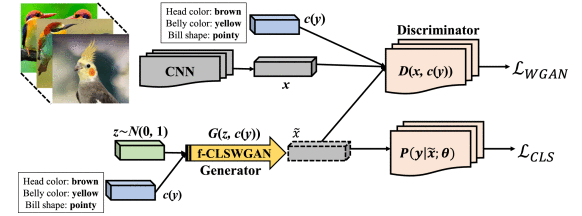
\includegraphics[width=1.1\textwidth,height=0.6\textheight,keepaspectratio]{script/f-CLSWGAN.PNG}
     	\end{center}
     	\begin{itemize}	
     		\item   It provides a measure of the discrepancy between predicted probabilities and true labels, and serves as an objective function to guide model training. By minimizing the negative log-likelihood loss, the model learns to make more accurate and confident predictions.
     	\end{itemize}
     	
     	
     \end{frame}
     
     
     
     	\begin{frame}[c,allowframebreaks]
     	\slideonly{\frametitle{Application : Generative-based methode(WGAN) }}
     	
     	\ndef{def:<label>}{wasserstein-distance and gradient penality}{
     		\begin{align*} \mathcal {L}_{WGAN}& =E[D(x^{s},a^{s})]-E[D(\tilde{x}^{s},a^{s})] \\ & \quad - \lambda E[(\Vert \bigtriangledown _{\hat{x}}D(\hat{x},a^{s})\Vert _{2}-1)^{2}],  \end{align*}
     		the difference between the expectation that the descriminator classifies real data as real and generated data as generated minus the gradient penality times the power $\lambda$ .
     		
     		\filledend}
     	\begin{itemize}	
     		\item  In addition, to generate discriminative features, the negative log-likelihood is used to minimize the classification loss	
     	\end{itemize}
     	
     	
     	
     	\frametitle{Satz \texttt{\symbol{92}nsatz} and
     		Theorem \texttt{\symbol{92}ntheorem}}
     	\sldown{0.5}
     	\nsatz{satz:ft}{negative \textsc{Log}-likelihood}{
     		
     		\slup{2}
     		\begin{align*} \mathcal {L}_{CLS}=-E_{\tilde{x}^{s}\sim p_{\tilde{x}^{s}}}[\log P(y^{s}|\tilde{x}^{s};\theta)], \tag{4} \end{align*}
     		\slup{2}}
     \end{frame}
     

	
	
			\begin{frame}[c,allowframebreaks]
		\slideonly{\frametitle{Application : Generative-based methode(WGAN) }}
		

		\ndef{def:<label>}{wasserstein GAN (WGAN)}{
		instead using the standard GAN Lossfunction, where the generator tries to deceive the descriminator, the wasserstein distance is used to stabilize the training and make it converges faster.
		
		\filledend}
	\ndef{def:<label>}{gradient penality}{
		ensure that the gradient of the descriminator on $\tilde{x}$(mix of real and generated data) satisfied the lipschitz condition , this penality is necessary to stabilize the convergence of the WGAN .
		\filledend}
		
			\sldown{0.5}
		
		
		\nsatz{satz:ft}{Lipschitz condition}{
			
			\slup{2}                                                            .\\                                                     
			 A function \( f: \mathbb{R}^n \to \mathbb{R}^m \) satisfies the Lipschitz condition if there exists a constant \( K \geq 0 \) such that for all \( x_1, x_2 \in \mathbb{R}^n \):
		
			 \[
			 \| f(x_1) - f(x_2) \| \leq K \| x_1 - x_2 \|
			 \]
			 	
			\slup{2}}
		
		
	\end{frame}
	
	
	
	
	
	
	
	
	

	
	
	
	\begin{frame}[c,allowframebreaks]
		\slideonly{\frametitle{Application : Generative-based methode(WGAN) }}
		
			\frametitle{Satz \texttt{\symbol{92}nsatz} and
			Theorem \texttt{\symbol{92}ntheorem}}
		\sldown{0.5}
		\nsatz{satz:ft}{negative \textsc{Log}-likelihood}{
			
			\slup{2}
			.\\
			The final objective function can be written as:
			\begin{align*} 
				\mathop{\min} _{G} \mathop{\max} _{D} \mathcal {L}_{WGAN}+\beta \mathcal {L}_{CLS}, \tag{5} \end{align*}
			\slup{2}}
			
		
			\begin{itemize}	
			\item The $\mathop{\min} _{G}$ : pushes the generator to minimize the WGANloss by generating a fake simple that resemble real data .\\
			$\mathop{\max} _{D} :$ pushes the descriminator to maximize the WGANloss by excluding the maximum of fake simple .
			
		\end{itemize}
		
	\end{frame}
	
	
	
	
	
	
\begin{frame}[c,allowframebreaks]
	\frametitle{Application: MDL4OW (Multitask Deep Learning)}
	
	\nblock{Problem}{
		In a closed-world setting, the existence of unknown or novel classes will lead to false positives, thereby reducing the precision of a model. The classifier tries to classify the unknown classes as seen classes because it cannot differentiate between known and unknown classes.
	}
	
	\nblock{Problem}{
		Let $X$ be the sample instance space. Each instance $x \in X$ is given a limited training set with index $k$, consisting of only a few samples $\left(x^k, l^k \right)$, where $l^k \in L = \{1, \ldots, |C|\}$ is the label index for $x^k$.
		
		The multilevel convolutional layers, along with batch normalization and the Rectified Linear Unit (ReLU), serve as a good encoder $\phi\left(\cdot\right)$ to extract the spectral-spatial features $x_{\phi}$ as the representation of the sample instance:
		
		\begin{tikzpicture}
			% Nodes
			\node[draw, ellipse] (ENCODER) at (0,0) {$\phi\left(\cdot\right)$};
			\node[draw, rectangle] (input) at (-2,0) {$x_{\phi_{conv}}$};
			\node[draw, rectangle] (output) at (2,0) {$x_{\phi_{conv}} = \phi_{conv}(x)$};
			
			% Arrows
			\draw[->] (input) -- (ENCODER);
			\draw[->] (ENCODER) -- (output);
		\end{tikzpicture}
	}
	
	\nblock{Definition: Normalized Inputs}{
		Normalization adjusts the values so they have a mean of $0$. This reduces fluctuations in the data (e.g., from $(-100, 500)$ to $(-1, 1)$), making the training process easier.
	}
		\nblock{Problem}{
			Then, the classifier $f\left(\cdot\right)$ takes the output vector $x_{\phi}$ from the feature extractor $\phi\left(\cdot\right)$ as its input. 
		 
			In a pure deep learning scenario,  the fully connected layer with the SoftMax activation function serves as the classifier $f(\cdot)$ and gives the probability $P\left(y=j | x_{\phi} \right)$ of the $j$-th category:
			\begin{equation}
				P \left(y=j|x_{\phi} \right) = \frac{\exp \left(x_{\phi}^T w_{j}+b_j \right)}{\sum_{c=1}^C{\exp \left(x_{\phi}^T w_c + b_c \right)}},
			\end{equation}
	
	
	}
	
      \end{frame}

	
	
	
	
	
	
	\begin{frame}[c,allowframebreaks]
		\slideonly{\frametitle{Application: MDL4OW (Multitask Deep Learning) }}
			\begin{itemize}	
			\item  $w_j$  is the weight vector of the j-th neuron in the fully
			connected layer
			\item $b_j$ is a bias element corresponding to the $j$-th neural
			
			\item $C$ is the number of the category
			
		\item	The classification task is to find the optimal parameters for  the network  by minimizing the   cross-entropy loss function  $\ell_c$:
		\end{itemize}
		\begin{equation}
			\ell_c \left(y,\hat{y} \right) =  - \sum_{i=1}^{C} y_i log \left(\hat{y}_i \right),
		\end{equation}
		\begin{itemize}
			\item  $C$ is the number of predefined classes
		\item $y$ is the ground truth label, and $\hat{y}$ is the predicted label.
 	\end{itemize}
		
		
	\end{frame}
	
	
	
	\begin{frame}[c,allowframebreaks]
		\slideonly{\frametitle{Application: MDL4OW (Multitask Deep Learning) }}
		\begin{itemize}	
			\item a naive solution to identify unknown classes is considering those instance with the largest probability smaller than 0.5 as unknown (softmax function with threshold= 0.5)
			\item the network cannot still identify the unknown. To empower the network with this ability, we add a reconstruction task:
			\begin{equation}
				\hat{x} = f_r \left(x_{\phi} \right),
			\end{equation}
		\item	$\hat{x}$ : the reconstructed instance
		\item $f_r \left(\cdot \right)$ the reconstruction function or named the decoder.
		\item $x_{\phi}$ is the output latent features from the encoder $\phi \left(\cdot \right)$. 
		\item the distance $\ell_1$ used as the reconstruction loss.
		\begin{equation}
			\ell_r \left(x, \hat{x} \right) = \left\Vert x - \hat{x} \right\Vert_1.
		\end{equation}
			
		\end{itemize}
		
	\end{frame}
	
	
	
	\begin{frame}[c,allowframebreaks]
		\slideonly{\frametitle{ Reconstruction via multitask learning }}
		\begin{itemize}	
		\item In the training phase for the multitask network, we minimize the total loss via backpropagation, 
		\begin{equation}
			\min\limits_{\phi\left(\cdot\right),f_c\left(\cdot\right),f_r\left(\cdot\right)} \lambda_c \ell_c \left(y, \hat{y} \right) + \lambda_r \ell_r \left(x, \hat{x} \right),
		\end{equation}
		$\lambda_c$ and $\lambda_r$ are the weights to control the loss influence on the multitask network for  $\ell_c$ and  $\ell_r$, respectively. 
		\item In the decoder, the key element is the deconvolutional layer can be considered as the inverse of  a convolutional layer, denoted as $\phi^{\dagger}_{conv} \left(\cdot \right)$, resulting:
		\begin{equation}
			x = \phi^{\dagger}_{conv} \left(\phi_{conv} \left(x \right) \right).
		\end{equation}
		
		
		
	    \end{itemize}
		
		
		
	\end{frame}
	
		\begin{frame}[c,allowframebreaks]
		\slideonly{\frametitle{DATASETS AND EXPERIMENTAL SETUP }}
		
			\nblock{Definition: open overall accuracy (OA)}{
			the proportion of corretly classified instances among all instances 
			\begin{equation} 
			\text{OA} = \frac{\text{Anzahl korrekt klassifizierter Instanzen}}{\text{Gesamtanzahl der Instanzen}}
		\end{equation}
			}
		\begin{itemize}	
			\item the value of the open  overall accuracy increased from 82.82 to 87.75 for the MDL4OW model compared to the close-world setting indicates that the MDL4OW model performs significantly better than the close-world .
		\end{itemize}
		\end{frame}
		
		
		
		
		
			\begin{frame}[c,allowframebreaks]
			\slideonly{\frametitle{evaluation metric }}
			
				\nblock{Definition: F1-score }{
				a balanced metric combining the Recal and precision .
				
				\begin{equation} 
					\text{F1-Score} = 2 \cdot \frac{\text{Precision} \cdot \text{Recall}}{\text{Precision} + \text{Recall}}
				\end{equation}
			}
			
		
			
			\nblock{Definition: Recall }{
			indicates the model ability to detect all relevant instances .
			
			\begin{equation} 
				\text{Recall} = \frac{\text{True Positives (TP)}}{\text{True Positives (TP)} + \text{False negative (FP)}}
			\end{equation}
		}
			
		\end{frame}
	
	
	
	
	
	
		\begin{frame}[c,allowframebreaks]
		\slideonly{\frametitle{ evaluation metric }}
		
			\nblock{Definition: precision }{
			indicates how many of the predicted instances are actualy correct.
			
			\begin{equation} 
				\text{Precision} = \frac{\text{True Positives (TP)}}{\text{True Positives (TP)} + \text{False Positives (FP)}}
			\end{equation}
		}
		
			\begin{itemize}	
			\item the value of F1-score decreased from 90.6 to 89.48 for the MDL4OW model compared to the close-world setting indicates a small drop in the balance between precision and recall in the open-world setting.
		\end{itemize}
		
		
			\nblock{Definition: Mapping error }{
			indicates the overall error in prediction the areas between the model's predicted area and the real actual area .
			
			\begin{equation} 
			\text{Errormax} = 2 \times \left(1 + \frac{A_{gt,C+1}}{\sum_{i=1}^{C} A_{gt,i}}\right)
			\end{equation}	
		}
		
		\begin{itemize}	
			\item $A_{gt,C+1}$ is the area of unknown class .
	    	\item	$\sum_{i=1}^{C} A_{gt,i}$ is the total sum of the area of the known classes.
	    	\item the value of Mapping error increased from 15.86 to 18.82 for the MDL4OW model compared to the close-world setting,which indicates that the model may have classified known class as unknown due the threshold (=0.5) used .
		\end{itemize}
	\end{frame}
	
	
	
	
	
		\begin{frame}[c,allowframebreaks]
		\slideonly{\frametitle{ Application: MDL4OW (Multitask Deep Learning) }}
			 \begin{figure}[h!]
				\centering
				\begin{minipage}{0.48\textwidth}
					\centering
					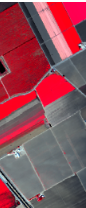
\includegraphics[width=1.1\textwidth,height=0.6\textheight,keepaspectratio]{script/Unbenannt.PNG}
				\end{minipage} 
				\hfill
				\begin{minipage}{0.48\textwidth}
					\centering
					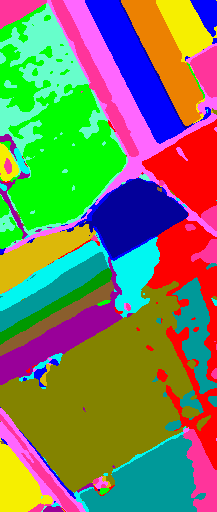
\includegraphics[width=1.1\textwidth,height=0.6\textheight,keepaspectratio]{script/salinas_close_0.png}
				\end{minipage}
			\end{figure}
		\begin{itemize}	
			\item   some of the materials are not represented in the training sample, for exemple, for the right image, the road and the houses between farmlands cannot be classified into any of the known classes.however,the closed model has it classified as combinaition of seen classes, which dosn't reflect the reality .
		\end{itemize}
		
	\end{frame}
	
	
	
	
		\begin{frame}[c,allowframebreaks]
		\slideonly{\frametitle{ Application: MDL4OW (Multitask Deep Learning)}}
		
		 \begin{figure}[h!]
			\centering
			\begin{minipage}{0.48\textwidth}
				\centering
				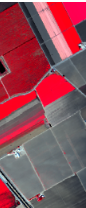
\includegraphics[width=1.1\textwidth,height=0.6\textheight,keepaspectratio]{script/Unbenannt.PNG}
			\end{minipage} 
			\hfill
			\begin{minipage}{0.48\textwidth}
				\centering
				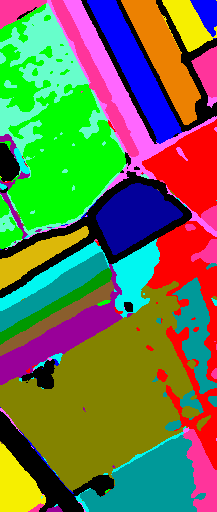
\includegraphics[width=1.1\textwidth,height=0.6\textheight,keepaspectratio]{script/salinas_mdl4ow_0.png}
			\end{minipage}
		\end{figure}
		\begin{itemize}	
			\item   by using the multitask deep learning the model has the ability to identify the unknown: the road and the hauses between farmlands (masked with black color) are succesfully identified .
		\end{itemize}
		
	\end{frame}
	
	
	
	
	
	
		\begin{frame}[c,allowframebreaks]
		\slideonly{\frametitle{ Reconstruction via multitask learning }}
		
		
	\end{frame}
	
	
	
	
	
		\begin{frame}[c,allowframebreaks]
		\slideonly{\frametitle{ Reconstruction via multitask learning }}
		
		
	\end{frame}
	
	
	
	
	
		\begin{frame}[c,allowframebreaks]
		\slideonly{\frametitle{ Reconstruction via multitask learning }}
		
		
	\end{frame}
	
	\framebreak %-----------------------------------------------------------------%
	
	
	


	
	
	
	
	
	
	\Uebung{ue:<uelabel1b>}{...}
	{
		...
		\begin{itemize}
			\item[a)] ...
			\item[b)] ...
			\item[c)] ...
		\end{itemize}          
	}
	



%------------------------------------EOF--------------------------------------%






